
    \documentclass[tikz,convert={outfile=\jobname.png}]{standalone}
    \usetikzlibrary{mindmap,trees,backgrounds}
    \usepackage{fontspec}
    \defaultfontfeatures{Ligatures=TeX,Scale=3}
    \setmainfont{M+ 1mn}
    
    
    \definecolor{red}{RGB}{228, 26, 28}
    \definecolor{blue}{RGB}{55, 126, 184}
    \definecolor{green}{RGB}{77, 175, 74}
    \definecolor{purple}{RGB}{152, 78, 163}
    \definecolor{orange}{RGB}{255, 127, 0}
    \definecolor{yellow}{RGB}{255, 255, 51}
    \definecolor{brown}{RGB}{166, 86, 40}
    \definecolor{black}{RGB}{0.0, 0.0, 0.0}
    \definecolor{dimgray}{RGB}{104.55, 104.55, 104.55}
    \definecolor{white}{RGB}{255.0, 255.0, 255.0}
    
    \begin{document}
    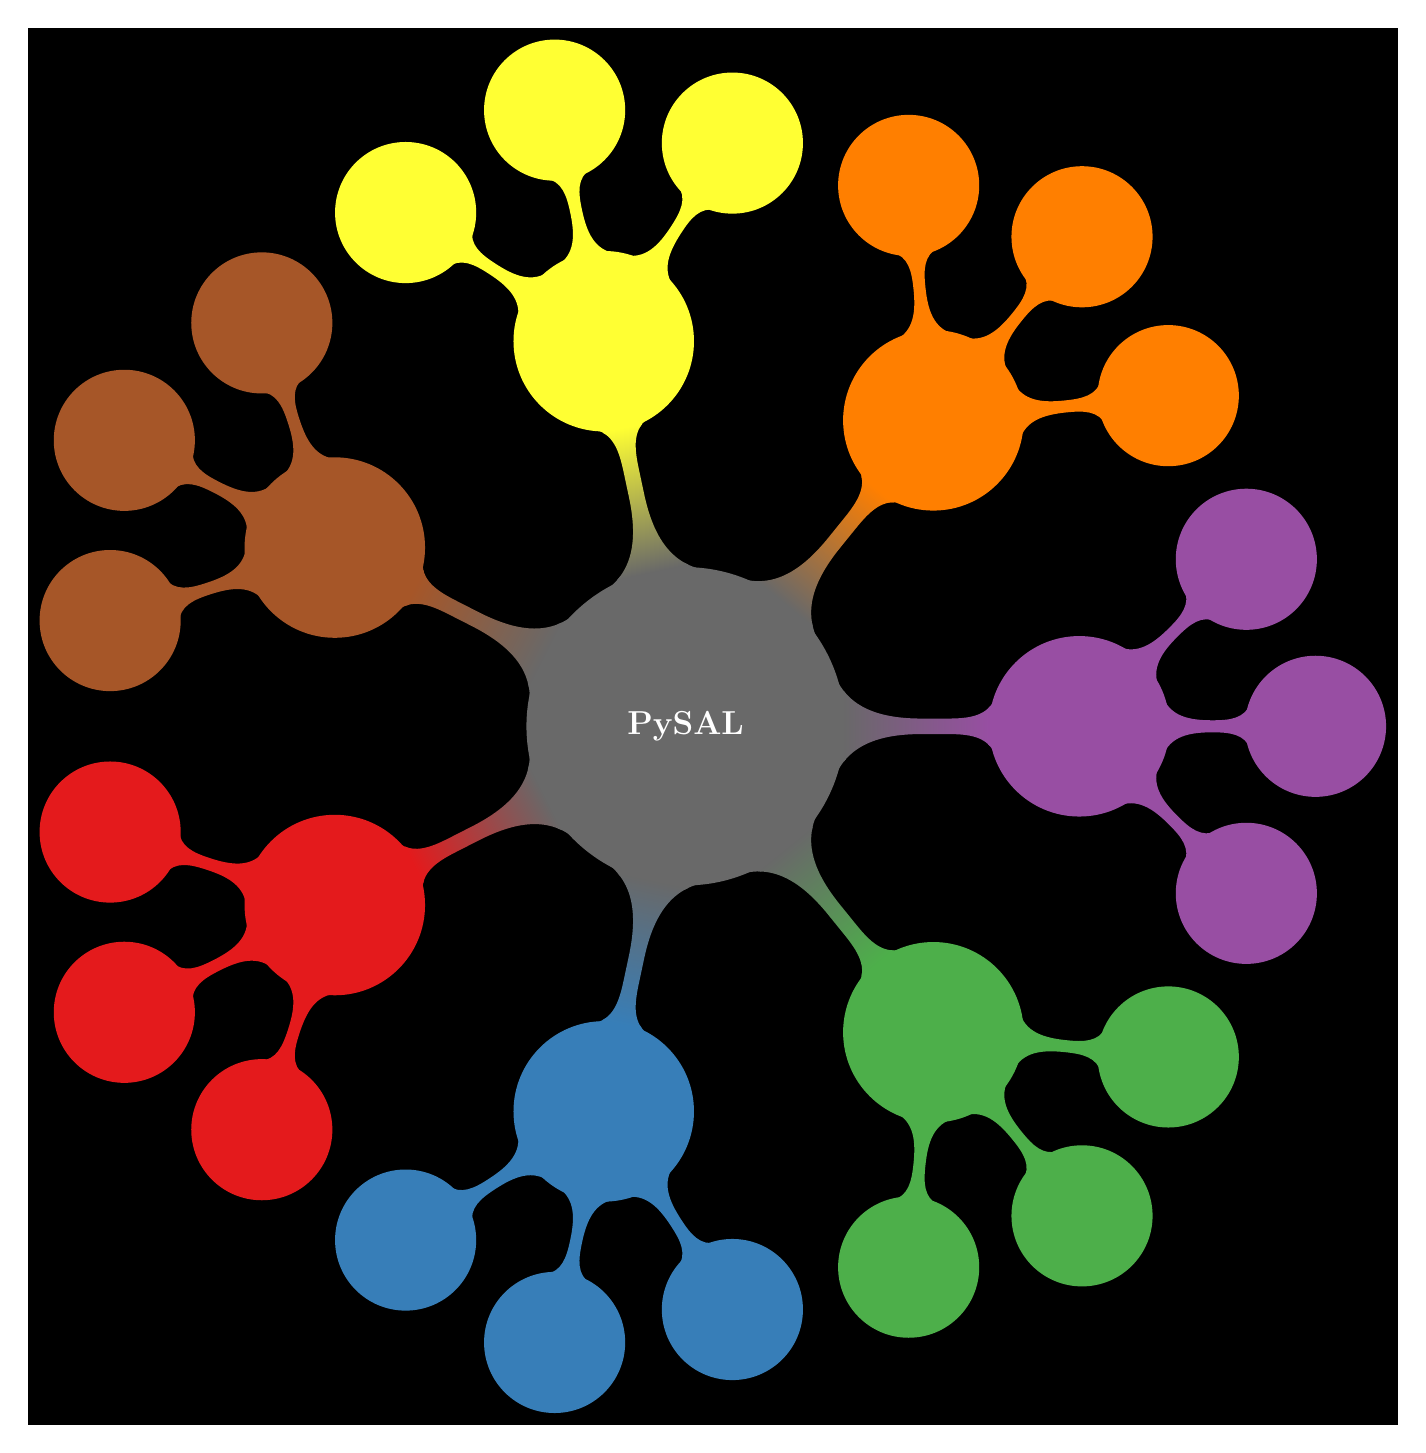
\begin{tikzpicture}[
        background rectangle/.style={fill=black},
        show background rectangle,
        mindmap,
        grow cyclic,
        every node/.style=concept,
        concept color=dimgray,
        text=white,
        level 1/.append style={
            level distance=5cm,
            sibling angle=51,
            font=\Huge
        },
        level 2/.append style={
            level distance=3cm,
            sibling angle=45
        }
    ]
    
        \node[concept color=dimgray]{\large\bfseries{PySAL}}
        child [concept color=red]{ node {}
            child { node { }}
            child { node { }}
            child { node { }}
         }
        child [concept color=blue]{ node {}
            child { node { }}
            child { node { }}
            child { node { }}
         }
        child [concept color=green]{ node {}
            child { node { }}
            child { node { }}
            child { node { }}
         }
        child [concept color=purple]{ node {}
            child { node { }}
            child { node { }}
            child { node { }}
         }
        child [concept color=orange]{ node {}
            child { node { }}
            child { node { }}
            child { node { }}
         }
        child [concept color=yellow]{ node {}
            child { node { }}
            child { node { }}
            child { node { }}
         }
        child [concept color=brown]{ node {}
            child { node { }}
            child { node { }}
            child { node { }}
         }
                ;
    \end{tikzpicture}
    \end{document}